\documentclass[10pt]{exam}
\usepackage[T1]{fontenc}
\usepackage[paper=a4paper,margin=2cm]{geometry}
\usepackage[sfdefault,light]{roboto}

\usepackage[usenames,dvipsnames]{xcolor}
\usepackage{amsmath,amssymb,array,graphicx,enumitem,listings,lstautogobble,multicol,textcomp,titlesec}
\usepackage{mathtools}

\setlength\parindent{0cm}

%Title & Section Formatting
\titleformat{\section}{\normalfont\Large\bfseries}{}{0em}{}[{\titlerule[0.5pt]}]
\titleformat{\subsection}{\normalfont\large\bfseries}{}{0em}{}

%Mathematical Shortcuts
\newcommand{\floor}[1]{\left\lfloor #1 \right\rfloor}
\newcommand{\ceil}[1]{\left\lceil #1 \right\rceil}

%Listings Shortcuts & Settings
\newcommand{\code}[1]{\lstinline{#1}}
\lstset{language=Java,
        autogobble=true,
        basicstyle=\ttfamily,
        commentstyle=\color{black!45},
        keywordstyle=\bfseries,
        showstringspaces=false,
        upquote=true}

%General Shortcuts
\newcommand{\blankpage}{\null\thispagestyle{empty}\addtocounter{page}{-1}\newpage}

\usepackage{draftwatermark,transparent}
\SetWatermarkAngle{0}
\SetWatermarkText{\transparent{0.025}\includegraphics[scale=0.75]{graphics/logo_black.png}}

%Color-Coded questions
\newcommand{\ColourQuestion}[3]{\renewcommand{\questionlabel}{\colorbox{#1}{\bfseries\color{white}\thequestion}\hfill}\question[#3] #2}
\newcommand{\BlueQuestion}[1]{\ColourQuestion{RoyalBlue}{#1}{1}}
\newcommand{\GreenQuestion}[1]{\ColourQuestion{ForestGreen}{#1}{2}}
\newcommand{\YellowQuestion}[1]{\ColourQuestion{Goldenrod}{#1}{4}}
\newcommand{\RedQuestion}[1]{\ColourQuestion{BrickRed}{#1}{6}}
\newcommand{\PurpleQuestion}[1]{\ColourQuestion{RoyalPurple}{#1}{30}}
\pointsinrightmargin

\header{\footnotesize\scshape Assignment \#\AssignmentNumber: \AssignmentTitle}{}{}
\cfoot{\footnotesize\scshape \AssignmentCourse\\Woodstock School---Mussoorie, Uttarakhand---India}


\def\AssignmentCourse{AP Computer Science Principles}
\def\AssignmentNumber{02}
\def\AssignmentTitle{Adding Colour}

\begin{document}
  \begin{questions}

    \BlueQuestion{With value ranges from $0$--$255$ for each colour, how many total possible colours can be expressed using the RGB colour model?}

    \BlueQuestion{Without programming them, describe the colours represented by each of the following.}\\
    {\small\textbf{Note:} This question is only looking for general descriptions of the colours.}
      \begin{parts}
        \part \code{fill(255, 0, 255);}
        \part \code{fill(0, 255, 255);}
        \part \code{fill(125, 125, 125);}
      \end{parts}

    %Add color to the Processing Bee!
    \GreenQuestion{Add colour to the Processing Bee from Assignment \#1.}\\
    {\small\textbf{Hint:} Yellow colours predominantly use red and green colour components, with blue being added to bring the colour closer to brown.}
      \begin{center}
        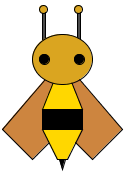
\includegraphics[scale=0.5]{files/ProcessingBeeColour}
      \end{center}

    \GreenQuestion{Why do you think the designers of the Processing language decided there was a need for both a grayscale \code{fill()} method as well an RGB model \code{fill()} method (which can easily be used to express various shades of gray)?}

    %Dart-Board Picture
    \RedQuestion{Use the Processing reference for the \code{arc()} drawing method (https://processing.org/reference/arc\_.html) to assist you in emulating the following image of a dartboard.\\
          {\small\textbf{Warning:} Using only the knowledge we have currently about the Processing language, this is a pretty long, tedious task; however, once you've determined how to draw the individual pieces of the board, the remaining pieces are not difficult to program.}\\
          {\small\textbf{Hint:} Because there are $20$ different ``wedges'' in the dart board, each arc should be $\frac{\pi}{5}$ radians wide.}
          \begin{center}
            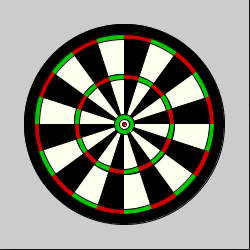
\includegraphics[scale=0.6]{files/DartBoard}
          \end{center}
    }
    
    \YellowQuestion{Explain the iterative process you took in creating your dart board program.}

  \end{questions}
\end{document}
